\section{提案手法}
SVMのハイパーパラメータ最適化では,カーネル関数の選択も考慮する余地があるが,カーネル関数を固定して行われた研究が多い.
本研究では,SVMのハイパーパラメータ$C$に加え,
(\ref{k1})〜(\ref{k4})式の4つのカーネル関数とそのハイパーパラメータ($\gamma$,coef0,$d$)
を最適化対象とする手法を提案する.
最適化アルゴリズムは設定パラメータの少ないABCを使用する.
これにより,ハイパーパラメータの探索範囲を広げ,より良いSVMモデルの探索が可能になる.
\subsection{ABCアルゴリズムの適用}
(\ref{k1})〜(\ref{k4})式の4つのカーネル関数は,ハイパーパラメータの数や性質が異なっている.
そのためカーネル関数が異なる個体では個体表現が変わり,個体の次元数が変化する.
しかし,(\ref{k2})〜(\ref{k4})式の$\gamma$や,
(\ref{k3}),(\ref{k4})式のcoef0はそれぞれスケール項,定数項と共通の性質を持っている.
そこで,本研究ではABCの個体表現を(\ref{expression})の5次元とし,
個体表現の変化をその個体の各次元の活性,非活性により表現することとした.
ここで,カーネル関数,$C$は常に使用されるハイパーパラメータで
$\gamma$,coef0,$d$はその個体のカーネル関数によって活性,非活性になる.
\begin{align}
    \text{個体表現:} \quad  (\text{カーネル関数},~C,~\gamma,~\text{coef0},~d)\label{expression}
\end{align}
カーネル関数の値は4つのカーネル関数を整数値にエンコードしたもので,
$C,~\gamma,~\text{coef0},~d$は[0.1]の範囲の実数とした.
得られた実数を$a$とするとそれぞれのパラメータは(\ref{map})式によって
指定した範囲内でSVMに適用する値$A$となる\cite{origin}.
ここで$a_{max}$,$a_{min}$はパラメータの上限値,下限値を表している.
\begin{align}
    \label{map}
    A =a(a_{max} -a_{min}) + a_{min}
\end{align}
また,$d$は離散値であるため,$A$を四捨五入したものをSVMに適用し,非活性の次元は探索の際に選択されない.
表~\ref{tab:param}にカーネル関数による活性,非活性の状態の組み合わせを示す.ここで1が活性,0が非活性を表す.
\begin{table}[t]
    \centering
    \caption{カーネル関数によるパラメータの活性,非活性}  % 表のキャプション
    \begin{tabular}{|c|c|c|c|}  % 3列を定義(c: 中央揃え、|: 縦線)
        \hline  % 横線
        カーネル関数 & $\gamma$ & coef0 & $d$\\  % ヘッダー行
        \hline  % 横線
        線形カーネル& 0& 0& 0\\  % 1行目
        \hline  % 横線
        RBFカーネル & 1 & 0& 0\\  % 2行目
        \hline  % 横線
        シグモイドカーネル & 1 & 1& 0\\  % 2行目
        \hline  % 横線
        多項式カーネル & 1 & 1& 1\\  % 2行目
        \hline  % 横線
    \end{tabular}
    
    \label{tab:param}  % 表のラベル
  \end{table} % 表のラベル
  
また,ABCによる最適化は連続値を前提としているため,
カテゴリ変数であるカーネル関数にABCの更新式は適用できない.
そこで本研究では更新次元にカーネル関数が選択された際の更新は
(\ref{karnel_update})式の確率$P$で更新されるものとする.
ここで$\boldsymbol{x_i}$は更新個体,
$\boldsymbol{x_j}$は$\boldsymbol{x_i}$と異なるカーネル関数を持つ個体の中からランダムに選ばれた個体である.
\begin{align}
    \label{karnel_update}
   P = \dfrac{f(\boldsymbol{x_j})}{f(\boldsymbol{x_i})+f(\boldsymbol{x_j})}
\end{align}

ABCにおける食物源の評価値$fit_i$は(\ref{fitness})式によって計算される.
ここで$miss_i$はSVMが検証セットの分類を行い,誤分類した割合である.
\begin{align}
    \label{fitness}
    fit_i = \dfrac{1}{1+miss_i}
\end{align}
\subsection{提案手法のアルゴリズム}
図~\ref{flowchart}にABCアルゴリズムによる最適化手順を示す.
\begin{figure}
    \centering
    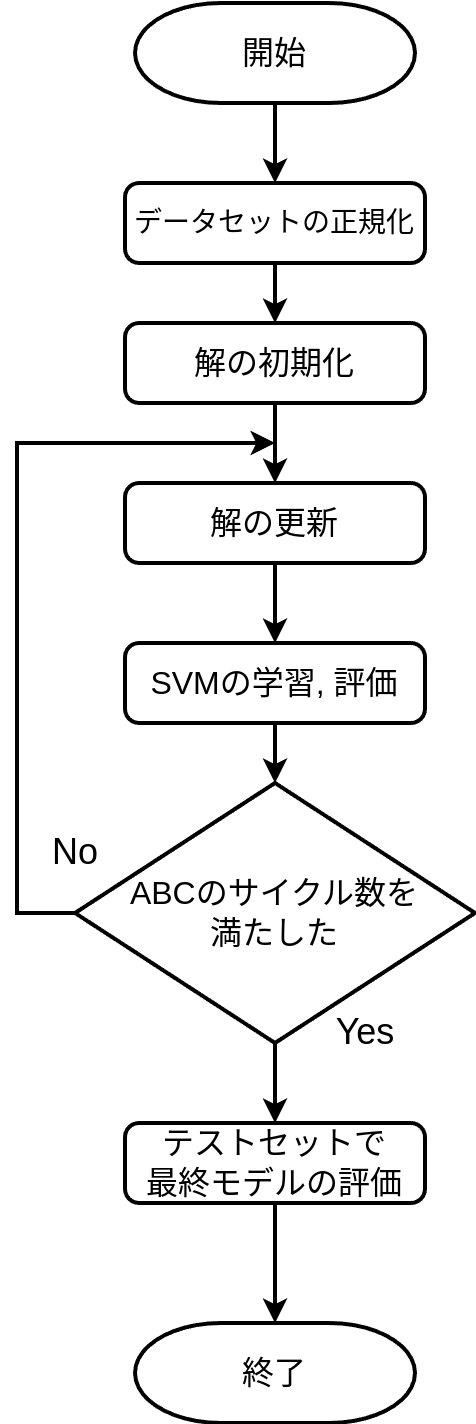
\includegraphics[width=0.4\linewidth]{flowchart.png}
    \caption{提案手法の最適化手順} 
    \label{flowchart}
\end{figure}
ABCアルゴリズムの詳細な手順を以下に示す.
ただし評価値の計算は次の手順で行われる.
\begin{enumerate}
    \item カーネル関数以外の値を(\ref{map})式でマッピング.
    \item その食物源が多項式カーネルだった場合$d$の値を四捨五入.
    \item 学習セットでsvmの学習を行う.
    \item 検証セットでsvmの分類精度を算出.
    \item (\ref{fitness})式で評価値の計算
\end{enumerate}

\subsubsection*{step 0 準備}
ABCにおけるパラメータである食物源の数$n$と探索上限回数$limit$の設定を行う.
次にSVNのハイパーパラメータ$C$,$\gamma$,coef0,$d$の探索範囲の設定を行い,
4つのカーネル関数を整数値にエンコードする.
最後に終了条件であるアルゴリズムのサイクル数を設定する.
\subsubsection*{step 1 初期化}
初期化では,$n$個の食物源をカーネル関数を定める1次元目を1〜4の整数値でランダムに初期化,
その他の2〜5次元は[0,1]の一様乱数で初期化する.
$n$個の食物源の評価値を計算し,
初期化された食物源の中で最も評価値が高い食物源
とそのインデックスを保存する.
\subsubsection*{step 2 収穫蜂フェーズ}
収穫蜂フェーズでは収穫蜂が食物源の近傍を探索する.
このときの更新式は(\ref{harvest})式のようになる.
ここで$j,k(k\neq i)$はランダムに選択される.
\begin{align}
v_{ij} = x_{ij} + rand[-1,1](x_{ij}-x_{kj})
\end{align}
ここで$v_{ij}$と$x_{ij}$の評価値を比較し,$v_{ij}$が$x_{ij}$よりも優れていたら$x_{ij}$を$v_{ij}$に置き換え,
$trial_i$を0にリセットする.
そうでなければ,$trial_i$を1増やす.
\subsubsection*{step 3 追従蜂フェーズ}
追従蜂フェーズでは収穫蜂フェーズによって更新された食物源の評価値に基づいて,
ルーレット選択を行い更新個体を選択する.
食物源$x_i$の選択確率$p_i$は(\ref{roulette})式のようになる.
そのため,評価値が高い食物源ほど選択確率が高く,評価値が低い食物源は選択確率が低くなる.
食物源の更新は収穫蜂フェーズと同様に行われる.
この操作を$n$回行う.
\begin{align}
    p_i = \dfrac{fit(\boldsymbol{x_{i}})}{\sum_{n}fit(\boldsymbol{x_{j}})}
\end{align}
\subsubsection*{step 3 追従蜂フェーズ}
追従蜂フェーズでは評価回数を減らすためにルーレット選択とは異なる手法に変更している.
各食物源$x_i$に対して1回ずつの更新確率$1 - p_i$で食物源の更新を行う.
食物源の更新は収穫蜂フェーズと同様に行われる.
確率未満の食料源は無視される.
この操作を$n$回行う.
そのため追従蜂の数は0〜nでランダムである.
\begin{align}
    p_i = \dfrac{fit(\boldsymbol{x_{i}})}{\sum_{n}fit(\boldsymbol{x_{j}})}
\end{align}
\subsubsection*{step 4 偵察蜂フェーズ}
偵察蜂フェーズでは,$trial$の値が探索打ち切り回数$limit$に達した
食物源をstep 1 の初期化と同じ手順でランダムな新たな解に置換する. 
置換した食物源の$trial$を0にリセットする.
$trial$の値が$limit$に達した
食物源がなければ何も行わない.
\subsubsection*{step 5 終了判定}
各食物源の評価値と,この時点で最良の食物源の評価値を比較し,
$fit(\boldsymbol{x_{i}}) > fit(\boldsymbol{x}_{best})$となる$\boldsymbol{x_{i}}$が存在する場合は
$\boldsymbol{x}_{best}$を更新する.
その後,指定したサイクル数を満たしていない場合は\textbf{step 2}に戻り,探索を続ける.
指定したサイクル数に達していた場合は,最適解をその時の$\boldsymbol{x}_{best}$として探索を終了し,
$\boldsymbol{x}_{best}$を適用したSVMモデルのテストセットに対する分類精度を算出する.